% Options for packages loaded elsewhere
\PassOptionsToPackage{unicode}{hyperref}
\PassOptionsToPackage{hyphens}{url}
\PassOptionsToPackage{dvipsnames,svgnames,x11names}{xcolor}
%
\documentclass[
  letterpaper,
  DIV=11,
  numbers=noendperiod]{scrartcl}

\usepackage{amsmath,amssymb}
\usepackage{lmodern}
\usepackage{iftex}
\ifPDFTeX
  \usepackage[T1]{fontenc}
  \usepackage[utf8]{inputenc}
  \usepackage{textcomp} % provide euro and other symbols
\else % if luatex or xetex
  \usepackage{unicode-math}
  \defaultfontfeatures{Scale=MatchLowercase}
  \defaultfontfeatures[\rmfamily]{Ligatures=TeX,Scale=1}
\fi
% Use upquote if available, for straight quotes in verbatim environments
\IfFileExists{upquote.sty}{\usepackage{upquote}}{}
\IfFileExists{microtype.sty}{% use microtype if available
  \usepackage[]{microtype}
  \UseMicrotypeSet[protrusion]{basicmath} % disable protrusion for tt fonts
}{}
\makeatletter
\@ifundefined{KOMAClassName}{% if non-KOMA class
  \IfFileExists{parskip.sty}{%
    \usepackage{parskip}
  }{% else
    \setlength{\parindent}{0pt}
    \setlength{\parskip}{6pt plus 2pt minus 1pt}}
}{% if KOMA class
  \KOMAoptions{parskip=half}}
\makeatother
\usepackage{xcolor}
\setlength{\emergencystretch}{3em} % prevent overfull lines
\setcounter{secnumdepth}{5}
% Make \paragraph and \subparagraph free-standing
\ifx\paragraph\undefined\else
  \let\oldparagraph\paragraph
  \renewcommand{\paragraph}[1]{\oldparagraph{#1}\mbox{}}
\fi
\ifx\subparagraph\undefined\else
  \let\oldsubparagraph\subparagraph
  \renewcommand{\subparagraph}[1]{\oldsubparagraph{#1}\mbox{}}
\fi

\usepackage{color}
\usepackage{fancyvrb}
\newcommand{\VerbBar}{|}
\newcommand{\VERB}{\Verb[commandchars=\\\{\}]}
\DefineVerbatimEnvironment{Highlighting}{Verbatim}{commandchars=\\\{\}}
% Add ',fontsize=\small' for more characters per line
\usepackage{framed}
\definecolor{shadecolor}{RGB}{241,243,245}
\newenvironment{Shaded}{\begin{snugshade}}{\end{snugshade}}
\newcommand{\AlertTok}[1]{\textcolor[rgb]{0.68,0.00,0.00}{#1}}
\newcommand{\AnnotationTok}[1]{\textcolor[rgb]{0.37,0.37,0.37}{#1}}
\newcommand{\AttributeTok}[1]{\textcolor[rgb]{0.40,0.45,0.13}{#1}}
\newcommand{\BaseNTok}[1]{\textcolor[rgb]{0.68,0.00,0.00}{#1}}
\newcommand{\BuiltInTok}[1]{\textcolor[rgb]{0.00,0.23,0.31}{#1}}
\newcommand{\CharTok}[1]{\textcolor[rgb]{0.13,0.47,0.30}{#1}}
\newcommand{\CommentTok}[1]{\textcolor[rgb]{0.37,0.37,0.37}{#1}}
\newcommand{\CommentVarTok}[1]{\textcolor[rgb]{0.37,0.37,0.37}{\textit{#1}}}
\newcommand{\ConstantTok}[1]{\textcolor[rgb]{0.56,0.35,0.01}{#1}}
\newcommand{\ControlFlowTok}[1]{\textcolor[rgb]{0.00,0.23,0.31}{#1}}
\newcommand{\DataTypeTok}[1]{\textcolor[rgb]{0.68,0.00,0.00}{#1}}
\newcommand{\DecValTok}[1]{\textcolor[rgb]{0.68,0.00,0.00}{#1}}
\newcommand{\DocumentationTok}[1]{\textcolor[rgb]{0.37,0.37,0.37}{\textit{#1}}}
\newcommand{\ErrorTok}[1]{\textcolor[rgb]{0.68,0.00,0.00}{#1}}
\newcommand{\ExtensionTok}[1]{\textcolor[rgb]{0.00,0.23,0.31}{#1}}
\newcommand{\FloatTok}[1]{\textcolor[rgb]{0.68,0.00,0.00}{#1}}
\newcommand{\FunctionTok}[1]{\textcolor[rgb]{0.28,0.35,0.67}{#1}}
\newcommand{\ImportTok}[1]{\textcolor[rgb]{0.00,0.46,0.62}{#1}}
\newcommand{\InformationTok}[1]{\textcolor[rgb]{0.37,0.37,0.37}{#1}}
\newcommand{\KeywordTok}[1]{\textcolor[rgb]{0.00,0.23,0.31}{#1}}
\newcommand{\NormalTok}[1]{\textcolor[rgb]{0.00,0.23,0.31}{#1}}
\newcommand{\OperatorTok}[1]{\textcolor[rgb]{0.37,0.37,0.37}{#1}}
\newcommand{\OtherTok}[1]{\textcolor[rgb]{0.00,0.23,0.31}{#1}}
\newcommand{\PreprocessorTok}[1]{\textcolor[rgb]{0.68,0.00,0.00}{#1}}
\newcommand{\RegionMarkerTok}[1]{\textcolor[rgb]{0.00,0.23,0.31}{#1}}
\newcommand{\SpecialCharTok}[1]{\textcolor[rgb]{0.37,0.37,0.37}{#1}}
\newcommand{\SpecialStringTok}[1]{\textcolor[rgb]{0.13,0.47,0.30}{#1}}
\newcommand{\StringTok}[1]{\textcolor[rgb]{0.13,0.47,0.30}{#1}}
\newcommand{\VariableTok}[1]{\textcolor[rgb]{0.07,0.07,0.07}{#1}}
\newcommand{\VerbatimStringTok}[1]{\textcolor[rgb]{0.13,0.47,0.30}{#1}}
\newcommand{\WarningTok}[1]{\textcolor[rgb]{0.37,0.37,0.37}{\textit{#1}}}

\providecommand{\tightlist}{%
  \setlength{\itemsep}{0pt}\setlength{\parskip}{0pt}}\usepackage{longtable,booktabs,array}
\usepackage{calc} % for calculating minipage widths
% Correct order of tables after \paragraph or \subparagraph
\usepackage{etoolbox}
\makeatletter
\patchcmd\longtable{\par}{\if@noskipsec\mbox{}\fi\par}{}{}
\makeatother
% Allow footnotes in longtable head/foot
\IfFileExists{footnotehyper.sty}{\usepackage{footnotehyper}}{\usepackage{footnote}}
\makesavenoteenv{longtable}
\usepackage{graphicx}
\makeatletter
\def\maxwidth{\ifdim\Gin@nat@width>\linewidth\linewidth\else\Gin@nat@width\fi}
\def\maxheight{\ifdim\Gin@nat@height>\textheight\textheight\else\Gin@nat@height\fi}
\makeatother
% Scale images if necessary, so that they will not overflow the page
% margins by default, and it is still possible to overwrite the defaults
% using explicit options in \includegraphics[width, height, ...]{}
\setkeys{Gin}{width=\maxwidth,height=\maxheight,keepaspectratio}
% Set default figure placement to htbp
\makeatletter
\def\fps@figure{htbp}
\makeatother
\newlength{\cslhangindent}
\setlength{\cslhangindent}{1.5em}
\newlength{\csllabelwidth}
\setlength{\csllabelwidth}{3em}
\newlength{\cslentryspacingunit} % times entry-spacing
\setlength{\cslentryspacingunit}{\parskip}
\newenvironment{CSLReferences}[2] % #1 hanging-ident, #2 entry spacing
 {% don't indent paragraphs
  \setlength{\parindent}{0pt}
  % turn on hanging indent if param 1 is 1
  \ifodd #1
  \let\oldpar\par
  \def\par{\hangindent=\cslhangindent\oldpar}
  \fi
  % set entry spacing
  \setlength{\parskip}{#2\cslentryspacingunit}
 }%
 {}
\usepackage{calc}
\newcommand{\CSLBlock}[1]{#1\hfill\break}
\newcommand{\CSLLeftMargin}[1]{\parbox[t]{\csllabelwidth}{#1}}
\newcommand{\CSLRightInline}[1]{\parbox[t]{\linewidth - \csllabelwidth}{#1}\break}
\newcommand{\CSLIndent}[1]{\hspace{\cslhangindent}#1}

\KOMAoption{captions}{tableheading}
\makeatletter
\makeatother
\makeatletter
\makeatother
\makeatletter
\@ifpackageloaded{caption}{}{\usepackage{caption}}
\AtBeginDocument{%
\ifdefined\contentsname
  \renewcommand*\contentsname{Table of contents}
\else
  \newcommand\contentsname{Table of contents}
\fi
\ifdefined\listfigurename
  \renewcommand*\listfigurename{List of Figures}
\else
  \newcommand\listfigurename{List of Figures}
\fi
\ifdefined\listtablename
  \renewcommand*\listtablename{List of Tables}
\else
  \newcommand\listtablename{List of Tables}
\fi
\ifdefined\figurename
  \renewcommand*\figurename{Figure}
\else
  \newcommand\figurename{Figure}
\fi
\ifdefined\tablename
  \renewcommand*\tablename{Table}
\else
  \newcommand\tablename{Table}
\fi
}
\@ifpackageloaded{float}{}{\usepackage{float}}
\floatstyle{ruled}
\@ifundefined{c@chapter}{\newfloat{codelisting}{h}{lop}}{\newfloat{codelisting}{h}{lop}[chapter]}
\floatname{codelisting}{Listing}
\newcommand*\listoflistings{\listof{codelisting}{List of Listings}}
\makeatother
\makeatletter
\@ifpackageloaded{caption}{}{\usepackage{caption}}
\@ifpackageloaded{subcaption}{}{\usepackage{subcaption}}
\makeatother
\makeatletter
\@ifpackageloaded{tcolorbox}{}{\usepackage[many]{tcolorbox}}
\makeatother
\makeatletter
\@ifundefined{shadecolor}{\definecolor{shadecolor}{rgb}{.97, .97, .97}}
\makeatother
\makeatletter
\makeatother
\ifLuaTeX
  \usepackage{selnolig}  % disable illegal ligatures
\fi
\IfFileExists{bookmark.sty}{\usepackage{bookmark}}{\usepackage{hyperref}}
\IfFileExists{xurl.sty}{\usepackage{xurl}}{} % add URL line breaks if available
\urlstyle{same} % disable monospaced font for URLs
\hypersetup{
  pdftitle={My title},
  pdfauthor={First author; Another author},
  colorlinks=true,
  linkcolor={blue},
  filecolor={Maroon},
  citecolor={Blue},
  urlcolor={Blue},
  pdfcreator={LaTeX via pandoc}}

\title{My title\thanks{Code and data are available at: LINK.}}
\usepackage{etoolbox}
\makeatletter
\providecommand{\subtitle}[1]{% add subtitle to \maketitle
  \apptocmd{\@title}{\par {\large #1 \par}}{}{}
}
\makeatother
\subtitle{My subtitle if needed}
\author{First author \and Another author}
\date{28 February 2023}

\begin{document}
\maketitle
\begin{abstract}
First sentence. Second sentence. Third sentence. Fourth sentence.
\end{abstract}
\ifdefined\Shaded\renewenvironment{Shaded}{\begin{tcolorbox}[interior hidden, enhanced, boxrule=0pt, borderline west={3pt}{0pt}{shadecolor}, breakable, sharp corners, frame hidden]}{\end{tcolorbox}}\fi

\begin{Shaded}
\begin{Highlighting}[]
\CommentTok{\#quarto references itself. wrapping in here:here goes in project }
\NormalTok{knitr}\SpecialCharTok{::}\FunctionTok{include\_graphics}\NormalTok{(here}\SpecialCharTok{::}\FunctionTok{here}\NormalTok{(}\StringTok{"inputs/data/apod\_20230227.jpg"}\NormalTok{))}
\end{Highlighting}
\end{Shaded}

\begin{figure}[H]

{\centering 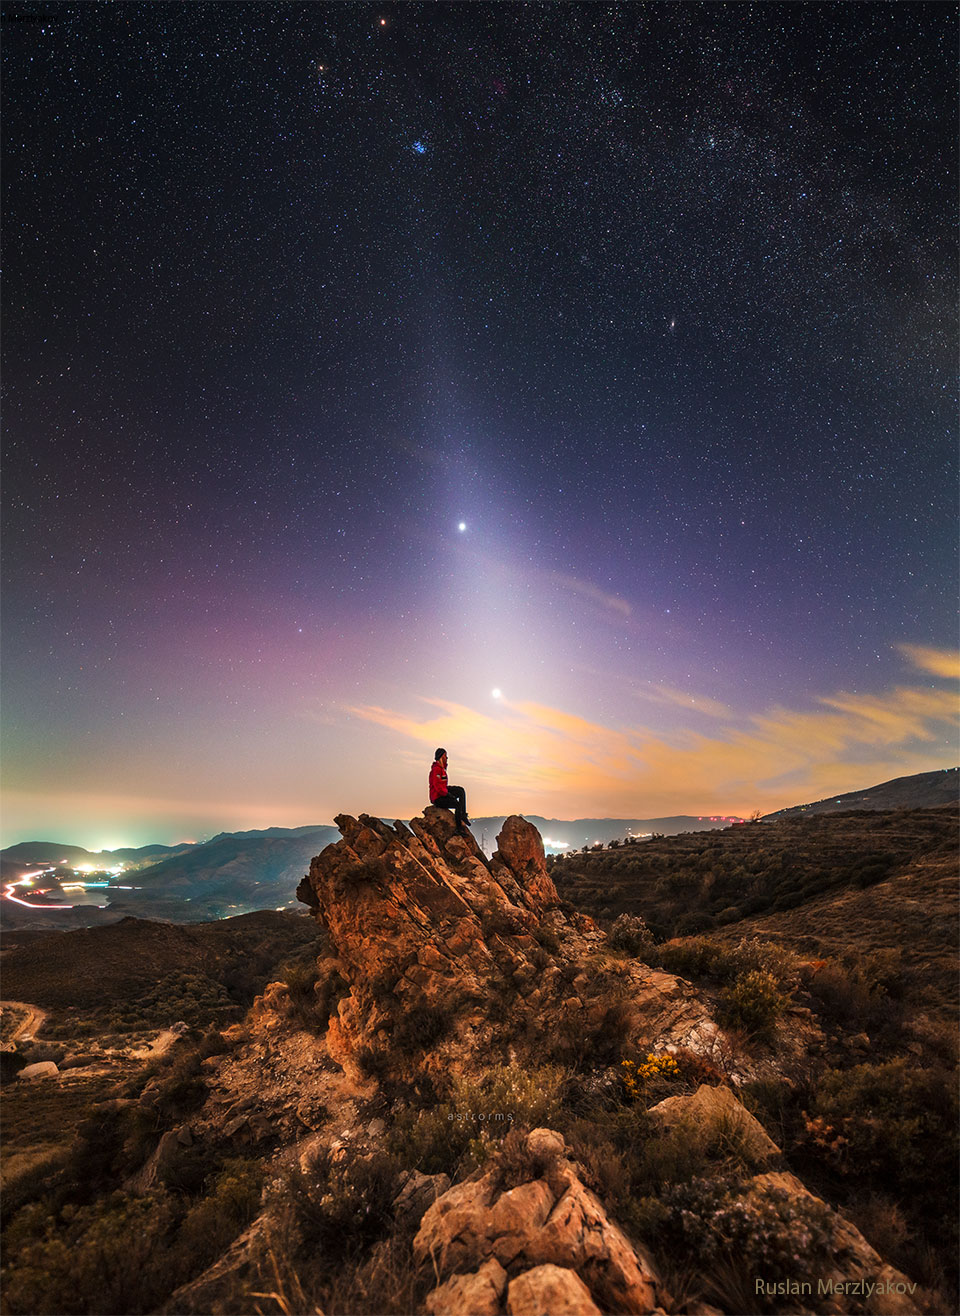
\includegraphics[width=3.2in,height=\textheight]{../../inputs/data/apod_20230227.jpg}

}

\end{figure}

\begin{verbatim}

Attaching package: 'lubridate'
\end{verbatim}

\begin{verbatim}
The following objects are masked from 'package:base':

    date, intersect, setdiff, union
\end{verbatim}

\begin{figure}

{\centering 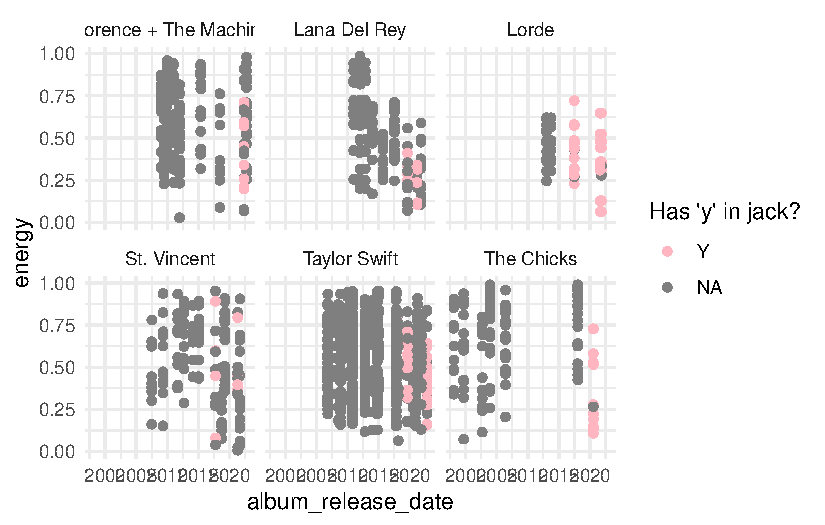
\includegraphics{paper_files/figure-pdf/fig-energy-1.pdf}

}

\caption{\label{fig-energy}Energy Variable}

\end{figure}

\begin{figure}

{\centering 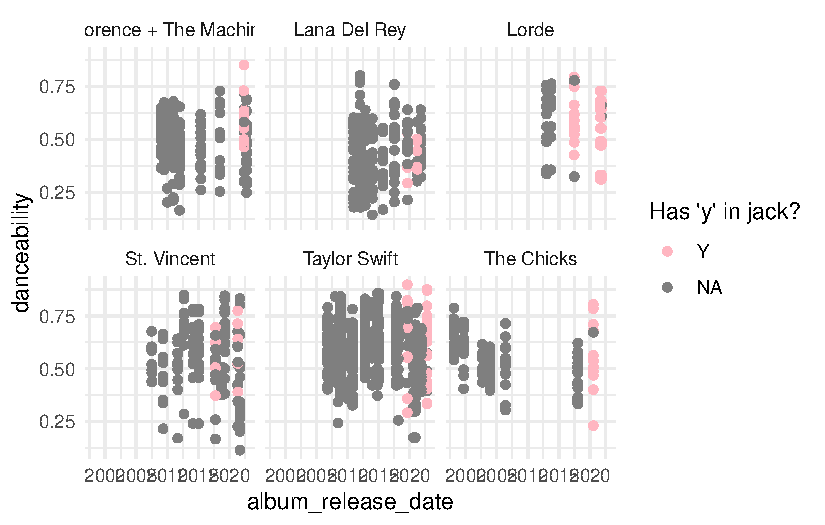
\includegraphics{paper_files/figure-pdf/fig-danceability-1.pdf}

}

\caption{\label{fig-danceability}Danceability Variable}

\end{figure}

\begin{figure}

{\centering 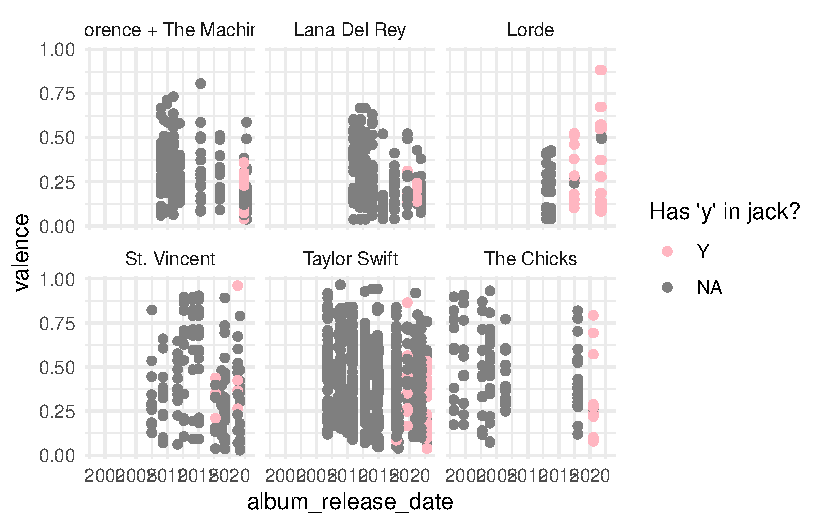
\includegraphics{paper_files/figure-pdf/fig-valence-1.pdf}

}

\caption{\label{fig-valence}Valence Variable}

\end{figure}

\begin{figure}

{\centering 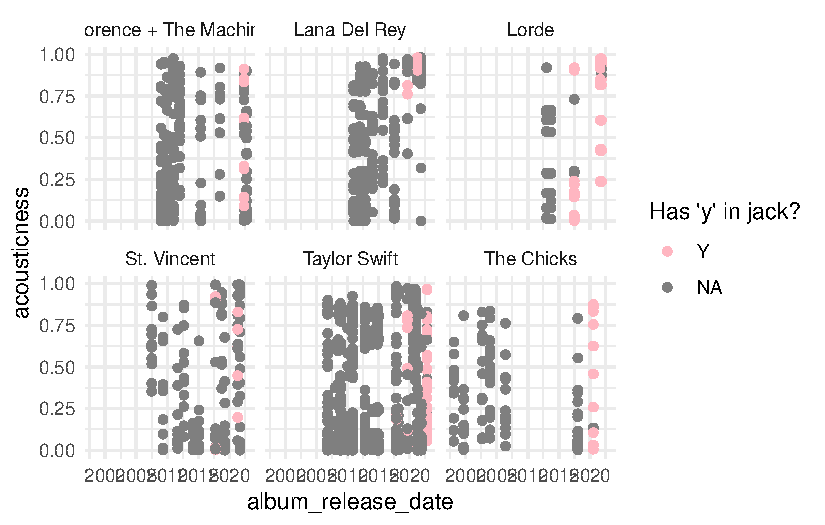
\includegraphics{paper_files/figure-pdf/fig-acousticness-1.pdf}

}

\caption{\label{fig-acousticness}Acousticness Variable}

\end{figure}

\begin{figure}

{\centering 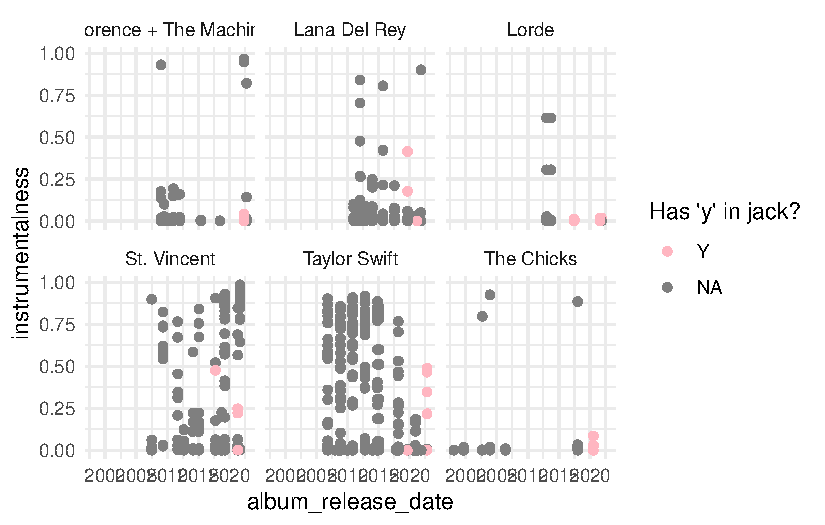
\includegraphics{paper_files/figure-pdf/fig-instrumentalness-1.pdf}

}

\caption{\label{fig-instrumentalness}Instrumentalness Variable}

\end{figure}

\begin{figure}

{\centering 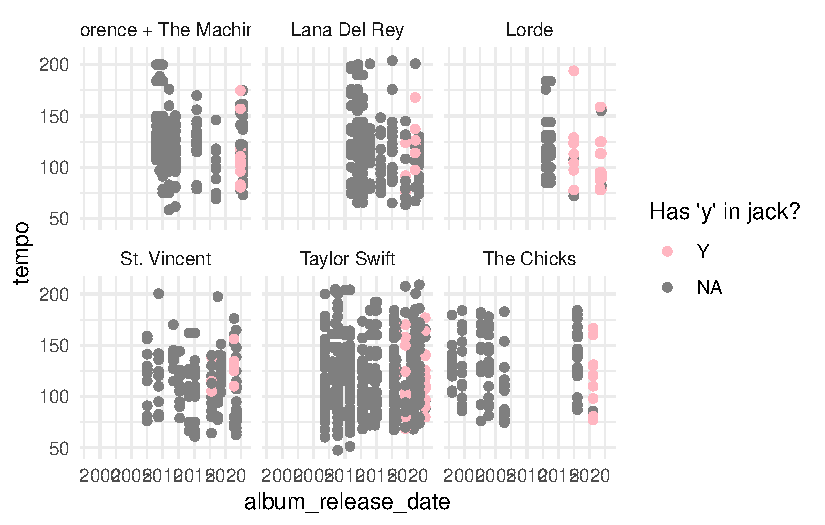
\includegraphics{paper_files/figure-pdf/fig-tempo-1.pdf}

}

\caption{\label{fig-tempo}Tempo Variable}

\end{figure}

\hypertarget{introduction}{%
\section{Introduction}\label{introduction}}

\hypertarget{sec-data}{%
\section{Data}\label{sec-data}}

\hypertarget{model}{%
\section{Model}\label{model}}

\begin{equation}\protect\hypertarget{eq-bayes}{}{
Pr(\theta | y) = \frac{Pr(y | \theta) Pr(\theta)}{Pr(y)}
}\label{eq-bayes}\end{equation}

Equation~\ref{eq-bayes} seems useful, eh?

Here's a dumb example of how to use some references: In paper we run our
analysis in \texttt{R} (R Core Team 2020). We also use the
\texttt{tidyverse} which was written by Wickham et al. (2019) If we were
interested in baseball data then Friendly et al. (2020) could be useful.

\hypertarget{results}{%
\section{Results}\label{results}}

\hypertarget{discussion}{%
\section{Discussion}\label{discussion}}

\hypertarget{sec-first-point}{%
\subsection{First discussion point}\label{sec-first-point}}

If my paper were 10 pages, then should be be at least 2.5 pages. The
discussion is a chance to show off what you know and what you learnt
from all this.

\hypertarget{second-discussion-point}{%
\subsection{Second discussion point}\label{second-discussion-point}}

\hypertarget{third-discussion-point}{%
\subsection{Third discussion point}\label{third-discussion-point}}

\hypertarget{weaknesses-and-next-steps}{%
\subsection{Weaknesses and next steps}\label{weaknesses-and-next-steps}}

Weaknesses and next steps should also be included.

\newpage

\appendix

\hypertarget{appendix}{%
\section*{Appendix}\label{appendix}}
\addcontentsline{toc}{section}{Appendix}

\hypertarget{additional-details}{%
\section{Additional details}\label{additional-details}}

\newpage

\hypertarget{references}{%
\section*{References}\label{references}}
\addcontentsline{toc}{section}{References}

\hypertarget{refs}{}
\begin{CSLReferences}{1}{0}
\leavevmode\vadjust pre{\hypertarget{ref-citeLahman}{}}%
Friendly, Michael, Chris Dalzell, Martin Monkman, and Dennis Murphy.
2020. \emph{Lahman: Sean {``Lahman''} Baseball Database}.
\url{https://CRAN.R-project.org/package=Lahman}.

\leavevmode\vadjust pre{\hypertarget{ref-citeR}{}}%
R Core Team. 2020. \emph{R: A Language and Environment for Statistical
Computing}. Vienna, Austria: R Foundation for Statistical Computing.
\url{https://www.R-project.org/}.

\leavevmode\vadjust pre{\hypertarget{ref-thereferencecanbewhatever}{}}%
Wickham, Hadley, Mara Averick, Jennifer Bryan, Winston Chang, Lucy
D'Agostino McGowan, Romain François, Garrett Grolemund, et al. 2019.
{``Welcome to the {tidyverse}.''} \emph{Journal of Open Source Software}
4 (43): 1686. \url{https://doi.org/10.21105/joss.01686}.

\end{CSLReferences}



\end{document}
